\section{Results}
\label{sec:results}

\para{Main result.}
\tabref{tab:main_results} reports primary metrics. The central pattern is that hidden categorical sampling behaves unlike output sampling. On \mnist, \hiddencategorical at $S=20$ reaches 79.41\% accuracy, compared with 98.55\% for deterministic inference and 98.51\% for \outputsample. On \fashionmnist, it reaches 66.30\%, compared with 88.77\% and 88.53\%. It also produces much higher \nll, \ece, entropy, and probability variance.

\begin{table}[t]
    \centering
    \caption{Primary test metrics. Accuracy is mean $\pm$ standard deviation across three seeds. Stochastic methods use $S=20$. Bold marks the best accuracy and lowest \nll/\ece within each dataset.}
    \label{tab:main_results}
    \resizebox{\textwidth}{!}{%
    \begin{tabular}{@{}lllrrrrr@{}}
        \toprule
        Dataset & Model & Method & Acc. (\%) & \nll & \ece & Entropy & Prob. var. \\
        \midrule
        \fashionmnist & deterministic & \deterministic & 88.77 $\pm$ 0.16 & 0.310 & 0.010 & 0.286 & 0.0000 \\
        \fashionmnist & deterministic & \gaussian & 88.75 $\pm$ 0.16 & 0.310 & {\bf 0.008} & 0.317 & 0.0013 \\
        \fashionmnist & deterministic & \hiddencategorical & 66.30 $\pm$ 13.40 & 1.032 & 0.202 & 1.464 & 0.0228 \\
        \fashionmnist & deterministic & \outputsample & 88.53 $\pm$ 0.13 & 0.734 & 0.015 & 0.249 & 0.0143 \\
        \fashionmnist & deterministic & \sap & 88.61 $\pm$ 0.03 & 0.320 & 0.024 & 0.371 & 0.0037 \\
        \fashionmnist & dropout & \dropouteval & {\bf 89.06 $\pm$ 0.36} & {\bf 0.305} & 0.008 & 0.282 & 0.0000 \\
        \fashionmnist & dropout & \mcdropout & 89.00 $\pm$ 0.25 & 0.307 & 0.009 & 0.328 & 0.0011 \\
        \midrule
        \mnist & deterministic & \deterministic & 98.55 $\pm$ 0.12 & 0.044 & 0.002 & 0.040 & 0.0000 \\
        \mnist & deterministic & \gaussian & 98.53 $\pm$ 0.12 & 0.044 & 0.003 & 0.053 & 0.0004 \\
        \mnist & deterministic & \hiddencategorical & 79.41 $\pm$ 9.27 & 0.833 & 0.254 & 1.304 & 0.0197 \\
        \mnist & deterministic & \outputsample & 98.51 $\pm$ 0.18 & 0.112 & 0.003 & 0.032 & 0.0019 \\
        \mnist & deterministic & \sap & 98.51 $\pm$ 0.12 & 0.055 & 0.017 & 0.100 & 0.0017 \\
        \mnist & dropout & \dropouteval & 98.81 $\pm$ 0.13 & {\bf 0.036} & {\bf 0.002} & 0.035 & 0.0000 \\
        \mnist & dropout & \mcdropout & {\bf 98.82 $\pm$ 0.14} & 0.038 & 0.006 & 0.059 & 0.0005 \\
        \bottomrule
    \end{tabular}}
\end{table}


\para{SAP and Gaussian sampling preserve accuracy.}
The less discrete hidden interventions are much less disruptive. On \mnist, \sap and \gaussian both remain within 0.04 percentage points of deterministic accuracy at $S=20$. On \fashionmnist, \sap is 0.15 points below deterministic accuracy and \gaussian is 0.02 points below. Their main visible effect is uncertainty: \sap increases entropy from 0.040 to 0.100 on \mnist and from 0.286 to 0.371 on \fashionmnist, while \gaussian increases entropy to 0.053 and 0.317.

\begin{figure}[t]
    \centering
    \begin{minipage}[b]{0.49\linewidth}
        \centering
        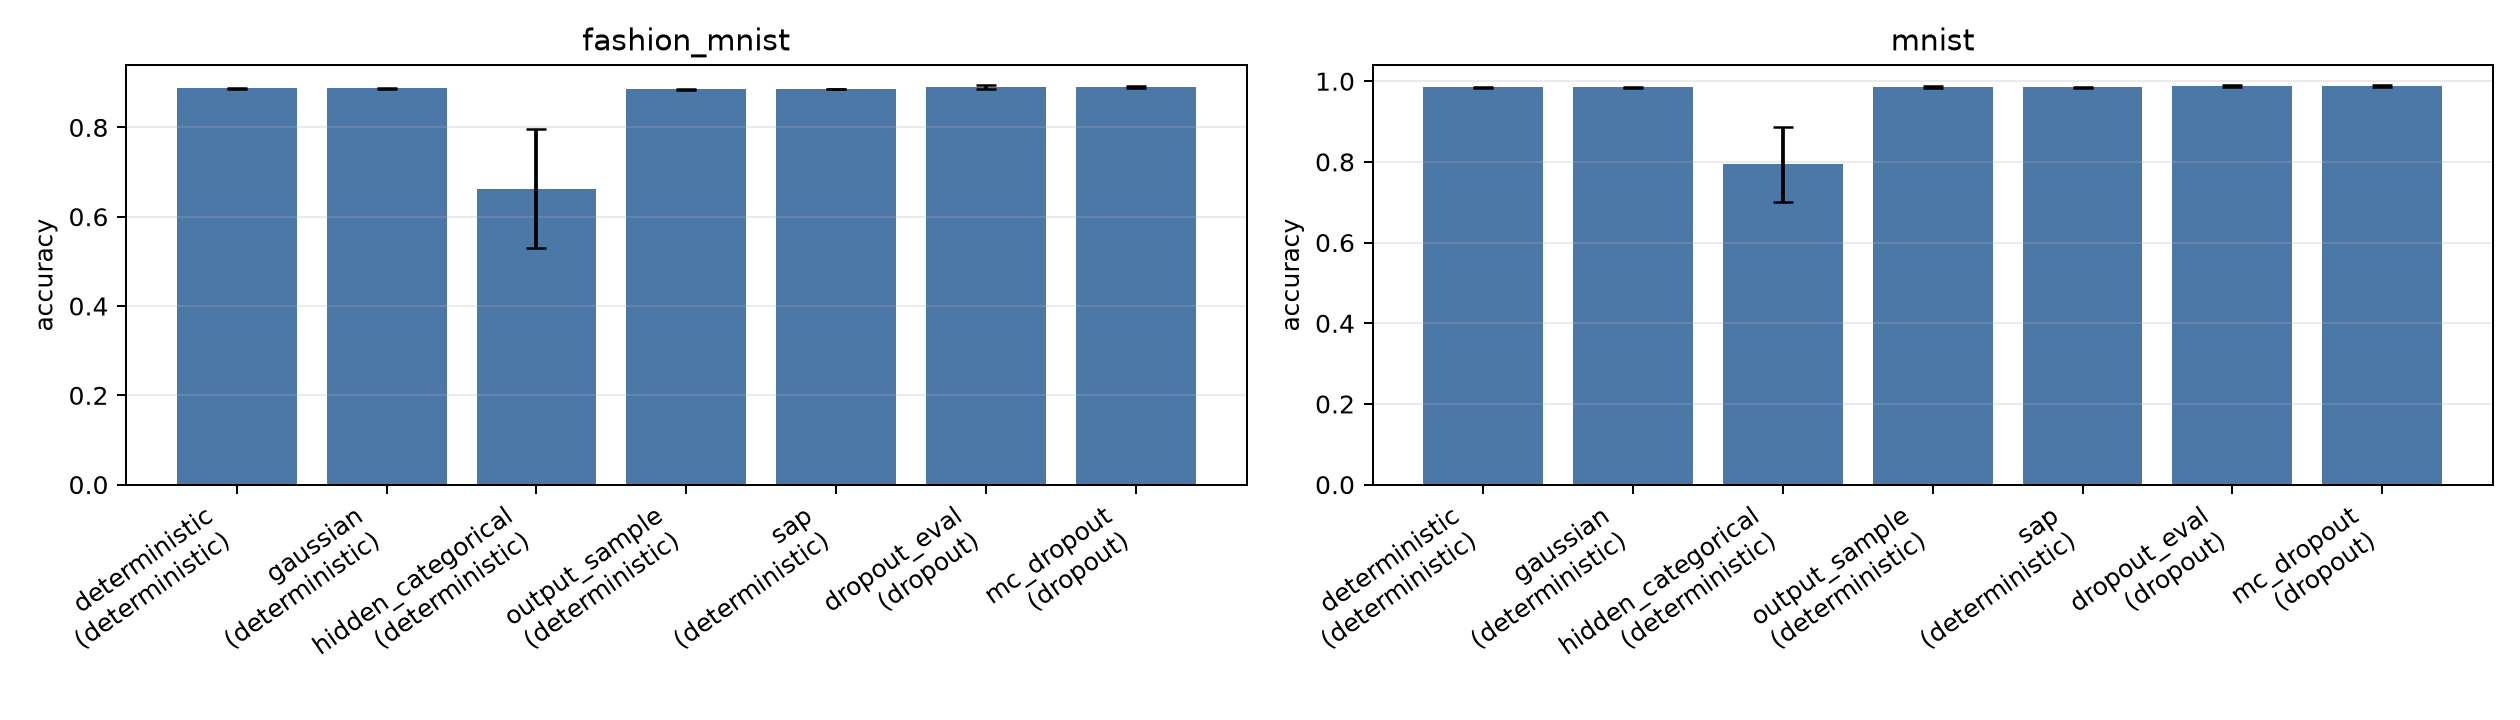
\includegraphics[width=\linewidth]{figures/accuracy_primary.png}
        \vspace{-0.7em}
        \centerline{\small (a) Accuracy}
    \end{minipage}
    \begin{minipage}[b]{0.49\linewidth}
        \centering
        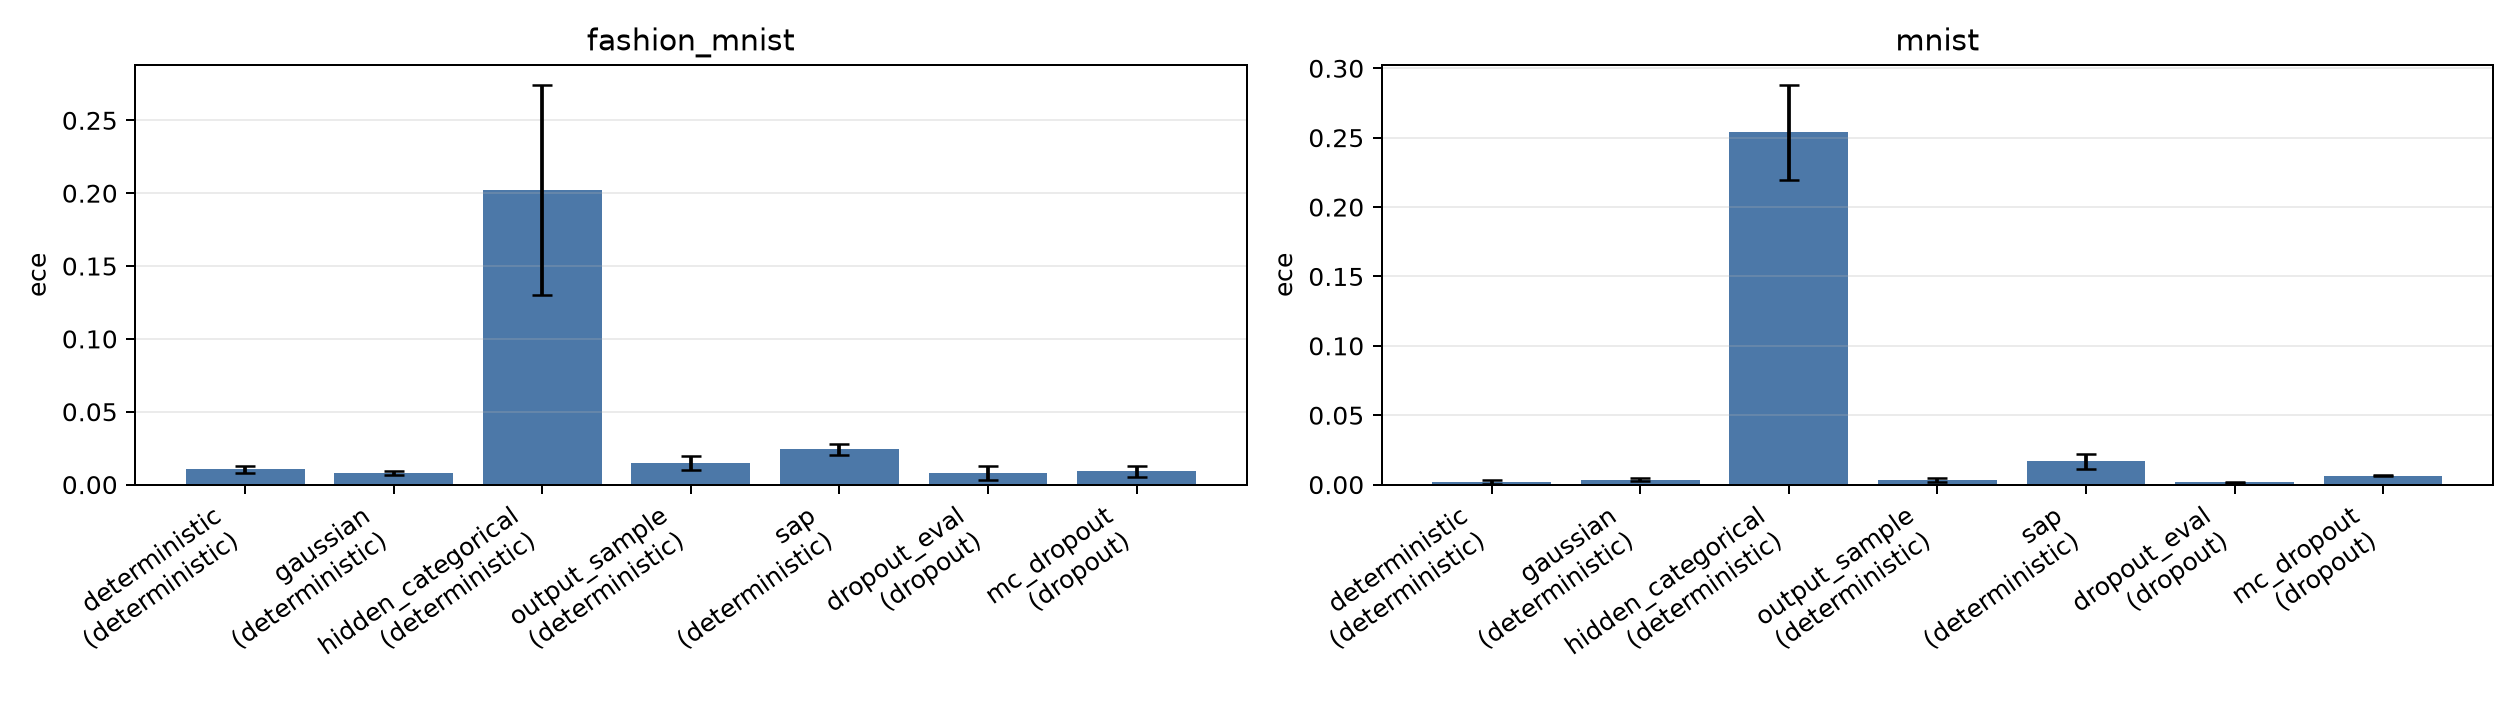
\includegraphics[width=\linewidth]{figures/ece_primary.png}
        \vspace{-0.7em}
        \centerline{\small (b) Expected calibration error}
    \end{minipage}
    \caption{Primary accuracy and calibration results. \hiddencategorical sharply reduces accuracy and increases \ece on both datasets. \sap, \gaussian, and \mcdropout preserve accuracy much more closely.}
    \label{fig:primary}
\end{figure}

\para{Output sampling is a readout-level intervention.}
Final-softmax sampling preserves top-line accuracy when $S$ is large enough because the underlying softmax probabilities are unchanged. However, the evaluated sampled distribution is a count distribution over 20 one-hot draws. This coarse empirical distribution worsens \nll from 0.044 to 0.112 on \mnist and from 0.310 to 0.734 on \fashionmnist, even though accuracy remains within 0.23 points of deterministic inference.

\para{Monte Carlo averaging helps but does not fix categorical hidden sampling.}
\tabref{tab:sample_count} shows the sample-count sweep. More samples improve every stochastic method, but the categorical hidden sampler remains far below deterministic inference. On \mnist, it rises from 62.28\% at $S=1$ to 79.41\% at $S=20$; on \fashionmnist, it rises from 50.06\% to 66.30\%. In contrast, \sap and \gaussian approach deterministic accuracy by $S=20$, and \mcdropout slightly improves the dropout-trained model's averaged prediction.

\begin{table}[t]
    \centering
    \caption{Accuracy across Monte Carlo sample counts. Values are mean $\pm$ standard deviation across three seeds. Increasing $S$ helps stochastic methods, but \hiddencategorical remains far below deterministic inference.}
    \label{tab:sample_count}
    \resizebox{\textwidth}{!}{%
    \begin{tabular}{@{}lllccc@{}}
        \toprule
        Dataset & Model & Method & $S=1$ & $S=5$ & $S=20$ \\
        \midrule
        \mnist & deterministic & \outputsample & 97.86 $\pm$ 0.19 & 98.39 $\pm$ 0.19 & 98.51 $\pm$ 0.18 \\
        \mnist & deterministic & \hiddencategorical & 62.28 $\pm$ 6.26 & 74.36 $\pm$ 8.36 & 79.41 $\pm$ 9.27 \\
        \mnist & deterministic & \sap & 97.22 $\pm$ 0.23 & 98.35 $\pm$ 0.07 & 98.51 $\pm$ 0.12 \\
        \mnist & deterministic & \gaussian & 98.20 $\pm$ 0.18 & 98.49 $\pm$ 0.11 & 98.53 $\pm$ 0.12 \\
        \mnist & dropout & \mcdropout & 98.44 $\pm$ 0.17 & 98.77 $\pm$ 0.18 & 98.82 $\pm$ 0.14 \\
        \midrule
        \fashionmnist & deterministic & \outputsample & 84.29 $\pm$ 0.40 & 87.58 $\pm$ 0.37 & 88.53 $\pm$ 0.13 \\
        \fashionmnist & deterministic & \hiddencategorical & 50.06 $\pm$ 7.19 & 60.52 $\pm$ 11.45 & 66.30 $\pm$ 13.40 \\
        \fashionmnist & deterministic & \sap & 86.04 $\pm$ 0.38 & 88.29 $\pm$ 0.20 & 88.61 $\pm$ 0.03 \\
        \fashionmnist & deterministic & \gaussian & 87.89 $\pm$ 0.14 & 88.66 $\pm$ 0.07 & 88.75 $\pm$ 0.16 \\
        \fashionmnist & dropout & \mcdropout & 88.23 $\pm$ 0.17 & 88.82 $\pm$ 0.17 & 89.00 $\pm$ 0.25 \\
        \bottomrule
    \end{tabular}}
\end{table}


\begin{figure}[t]
    \centering
    \begin{minipage}[b]{0.32\textwidth}
        \centering
        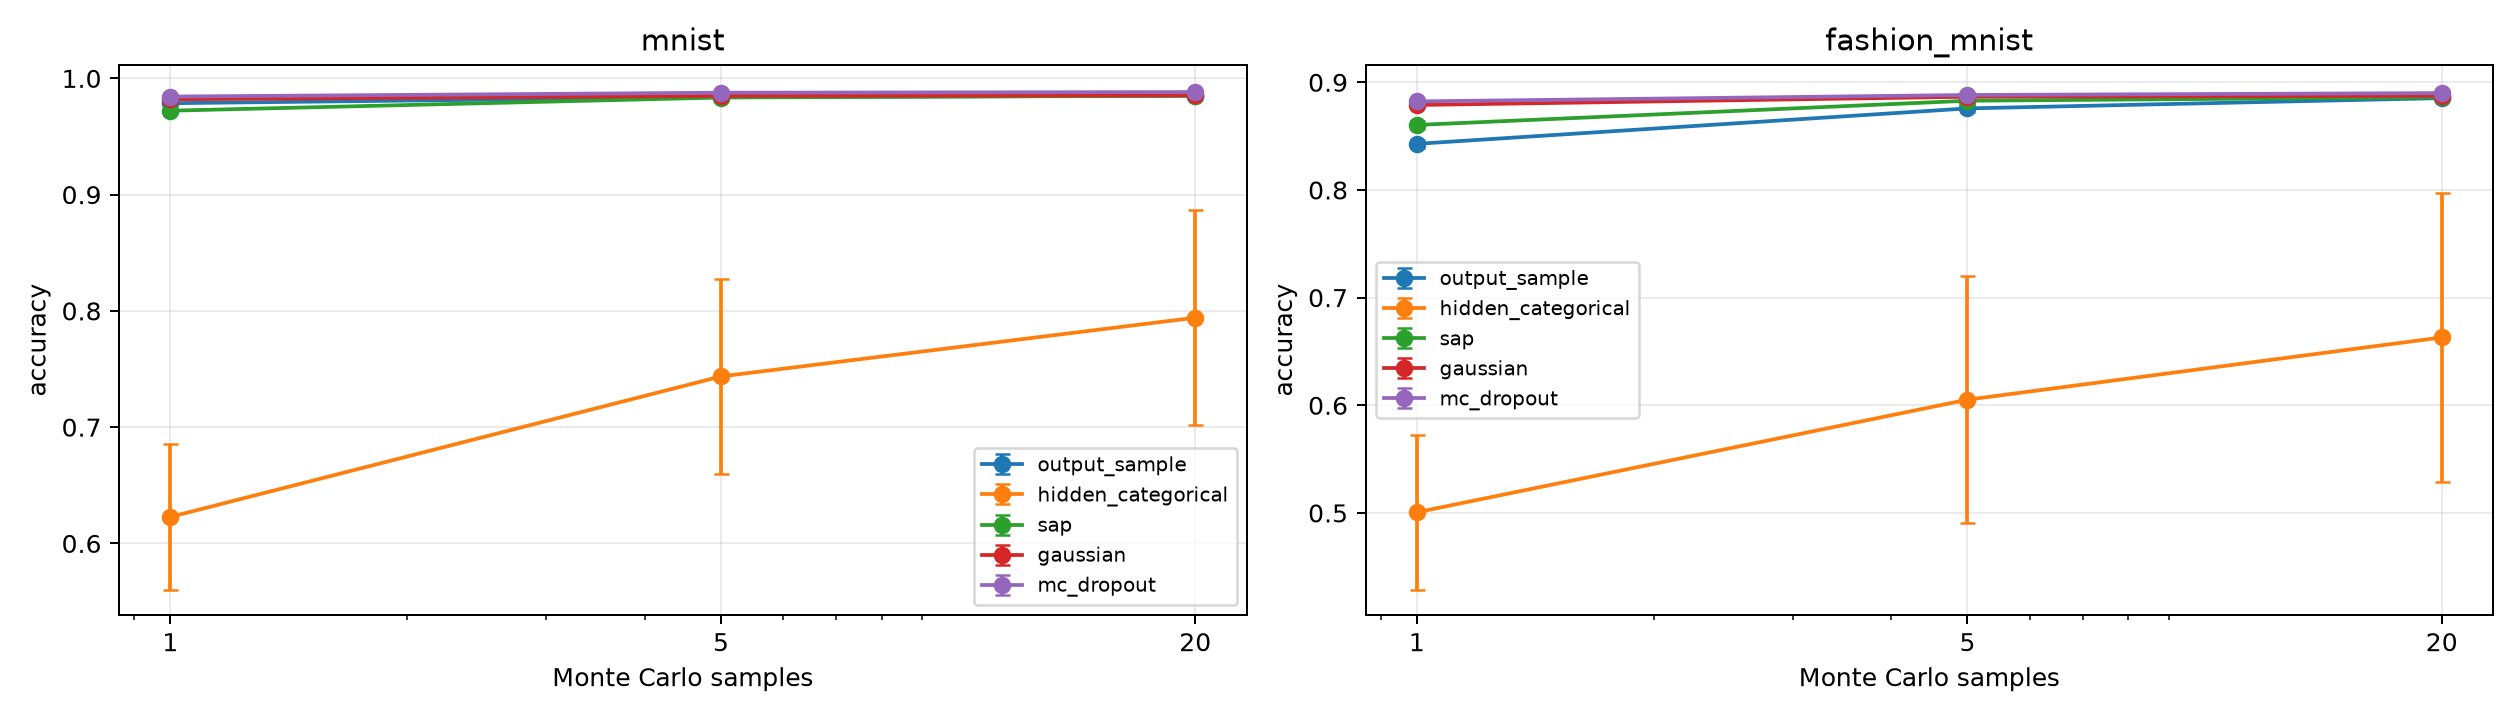
\includegraphics[width=\linewidth]{figures/accuracy_sample_sweep.png}
        \vspace{-0.7em}
        \centerline{\small (a) Accuracy}
    \end{minipage}
    \begin{minipage}[b]{0.32\textwidth}
        \centering
        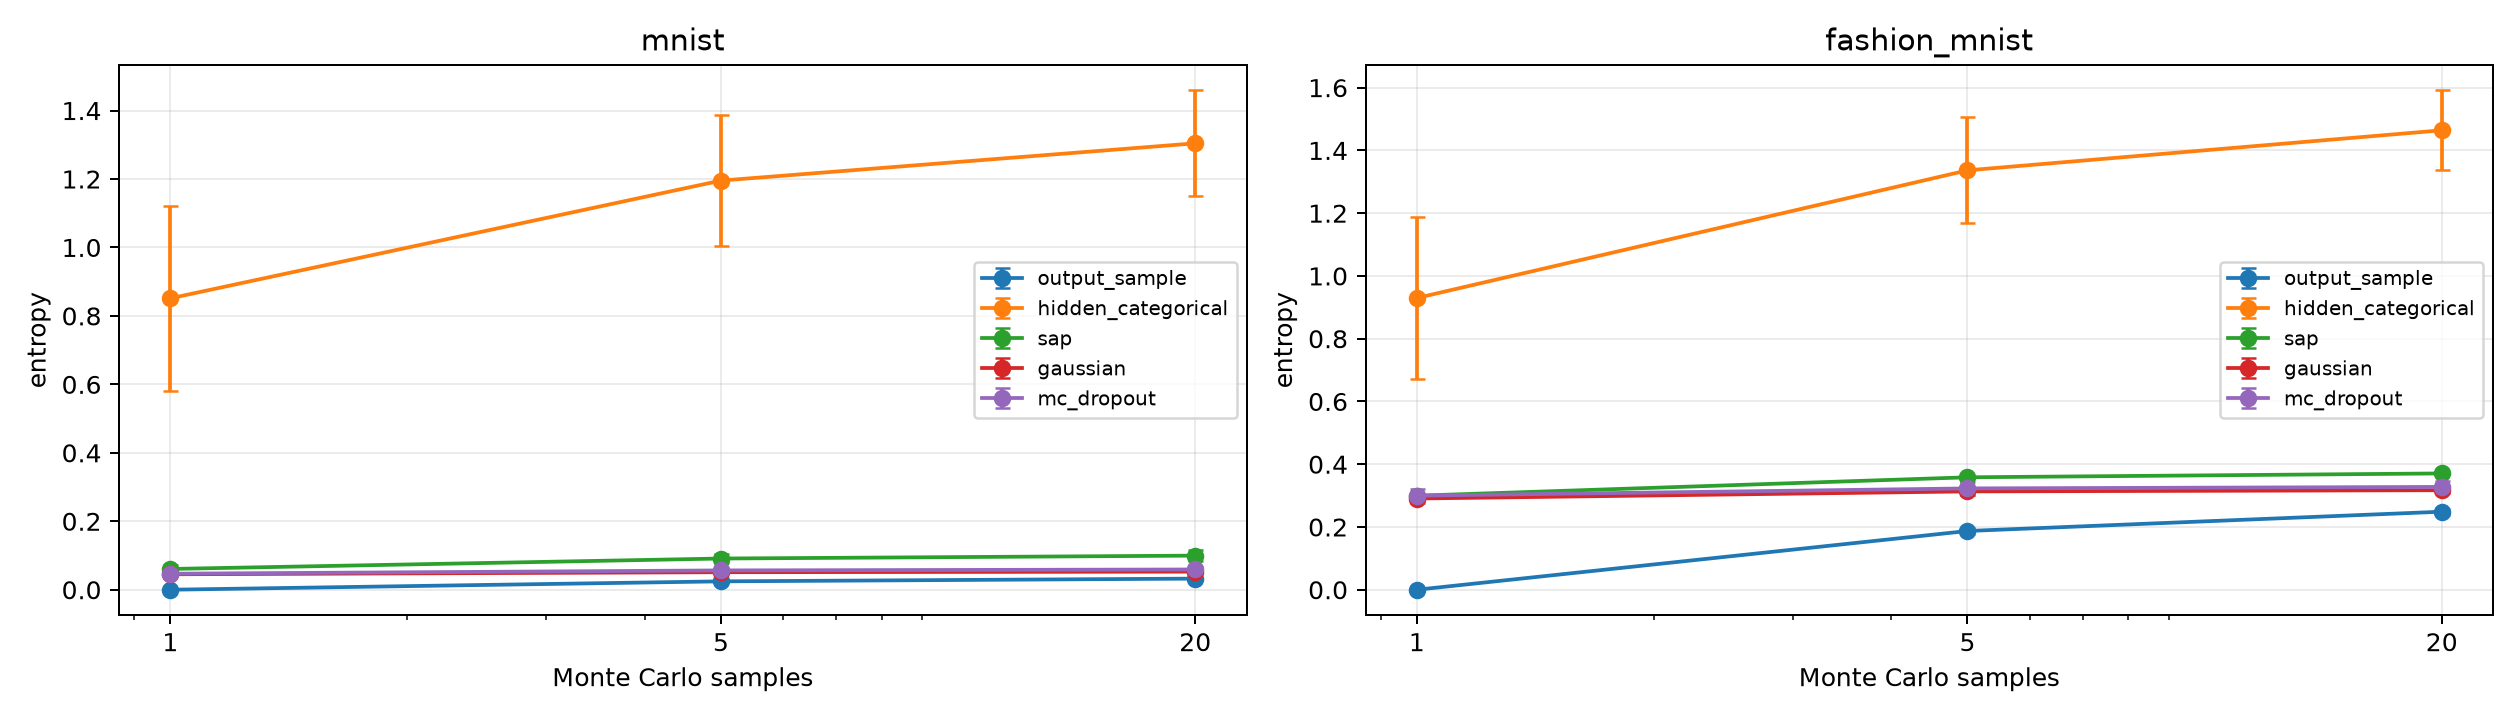
\includegraphics[width=\linewidth]{figures/entropy_sample_sweep.png}
        \vspace{-0.7em}
        \centerline{\small (b) Entropy}
    \end{minipage}
    \begin{minipage}[b]{0.32\textwidth}
        \centering
        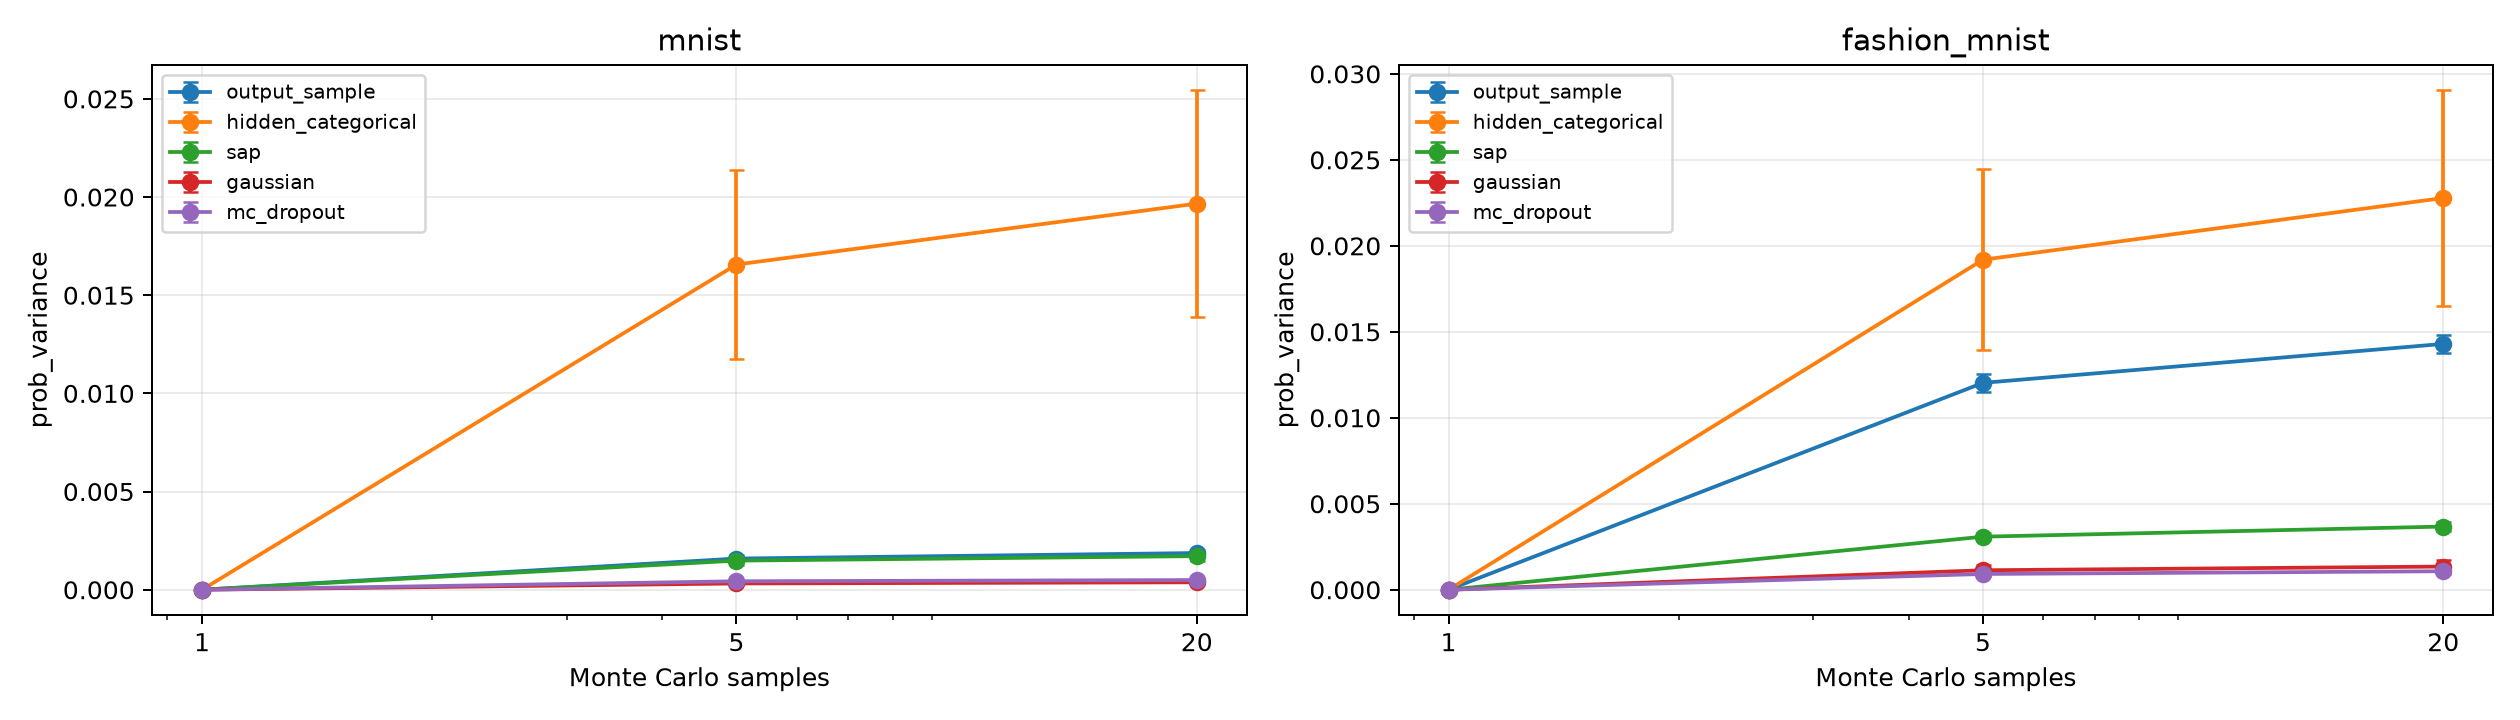
\includegraphics[width=\linewidth]{figures/variance_sample_sweep.png}
        \vspace{-0.7em}
        \centerline{\small (c) Probability variance}
    \end{minipage}
    \caption{Sample-count effects for stochastic inference. Monte Carlo averaging stabilizes predictions, but \hiddencategorical remains high-entropy and low-accuracy even at $S=20$.}
    \label{fig:sample_sweep}
\end{figure}

\para{Paired statistical comparisons.}
\tabref{tab:paired_differences} summarizes key paired differences against deterministic inference for deterministic-model methods at $S=20$. \hiddencategorical lowers accuracy by 19.13 percentage points on \mnist and 22.46 points on \fashionmnist. These accuracy differences have large paired effect sizes ($d_z=-2.07$ and $-1.66$), although Holm-corrected $p$-values are not below 0.05 with only three seeds. Calibration and entropy shifts are more consistent: \hiddencategorical increases \ece by 0.252 on \mnist ($p_{\mathrm{Holm}}=0.026$) and entropy by 1.265 on \mnist ($p_{\mathrm{Holm}}=0.015$) and 1.178 on \fashionmnist ($p_{\mathrm{Holm}}=0.011$).

\begin{table}[t]
    \centering
    \caption{Key paired differences versus deterministic inference for deterministic-model methods at $S=20$. Accuracy differences are percentage points; other differences are raw metric units. Holm-corrected $p$-values are descriptive because $n=3$ seeds.}
    \label{tab:paired_differences}
    \resizebox{\textwidth}{!}{%
    \begin{tabular}{@{}llrrrr@{}}
        \toprule
        Dataset & Method & $\Delta$ Acc. & $\Delta$ \nll & $\Delta$ \ece & $\Delta$ Entropy \\
        \midrule
        \mnist & \gaussian & -0.01 & 0.001 & 0.001 & 0.013 \\
        \mnist & \hiddencategorical & -19.13 & 0.789 & 0.252 & 1.265 \\
        \mnist & \outputsample & -0.03 & 0.069 & 0.001 & -0.007 \\
        \mnist & \sap & -0.03 & 0.011 & 0.015 & 0.060 \\
        \midrule
        \fashionmnist & \gaussian & -0.02 & 0.001 & -0.002 & 0.031 \\
        \fashionmnist & \hiddencategorical & -22.46 & 0.723 & 0.192 & 1.178 \\
        \fashionmnist & \outputsample & -0.23 & 0.424 & 0.004 & -0.037 \\
        \fashionmnist & \sap & -0.15 & 0.010 & 0.014 & 0.085 \\
        \bottomrule
    \end{tabular}}
\end{table}

